\section{Calculating The Vector}

% =================================
% SOLVING THE EQUATION
% =================================
\subsection{Solving the equation}

As mentioned before, we do now set the two functions equal to each other, to find the intersection point where the two functions meet – or in other words: Where the arrow actually hits the enemy.

\begin{eqnarray*}
        \overrightarrow{p}_{player} = {\begin{pmatrix} p_x \\ p_y \\ p_z \end{pmatrix}} & \coloneqq & \textit{the player's head position} \\
        \overrightarrow{d}_{proj} = {\begin{pmatrix} d_x \\ d_y \\ d_z \end{pmatrix}} & \coloneqq & \textit{the normalized direction of the projectile} \\
        v_{proj} & \coloneqq & \textit{the initial speed of the projectile} \\
        r_{proj} & \coloneqq & \textit{the air resistance constant for that specific projectile} \\
        g_{proj} & \coloneqq & \textit{the gravitational constant for that specific projectile} \\
        \overrightarrow{p}_{enemy} = {\begin{pmatrix} e_x \\ e_y \\ e_z \end{pmatrix}} & \coloneqq & \textit{the enemy's head position} \\
        \overrightarrow{v}_{enemy} = {\begin{pmatrix} v_{x_e} \\ v_{y_e} \\ v_{z_e} \end{pmatrix}} & \coloneqq & \textit{the current velocity of the enemy in x and z direction} \\
\end{eqnarray*}

\begin{equation*}
    \overrightarrow{s}_{enemy}(t) = \overrightarrow{s}_{proj}({\begin{pmatrix} d_x \\ d_y \\ d_z \end{pmatrix}}, t)
\end{equation*}

When solving this equation for the arrow vector, we get the three coordinates that define the exact direction where we have to shoot the arrow depending on the time we want the arrow to travel. We will handle this dependency later on. 

\begin{eqnarray*}
    {\begin{pmatrix} e_x \\ e_y \\ e_z \end{pmatrix}} + {\begin{pmatrix} v_{x_e} \\ v_{y_e} \\ v_{z_e} \end{pmatrix}} \cdot t & = & {\begin{pmatrix} p_x \\ p_y \\ p_z \end{pmatrix}} + \sum_{i=0}^{t-1} ({\begin{pmatrix} d_x \\ d_y \\ d_z \end{pmatrix}} \cdot v_{proj_0} \cdot r_{proj}^i - \sum_{k = 0}^{i - 1}({\begin{pmatrix} 0 \\ g_{proj} \\ 0 \end{pmatrix}} \cdot r^k))
    \\
    \Leftrightarrow {\begin{pmatrix} e_x \\ e_y \\ e_z \end{pmatrix}} + {\begin{pmatrix} v_{x_e} \\ v_{y_e} \\ v_{z_e} \end{pmatrix}} \cdot t & = & {\begin{pmatrix} p_x \\ p_y \\ p_z \end{pmatrix}} + \sum_{i=0}^{t-1} ({\begin{pmatrix} d_x \\ d_y \\ d_z \end{pmatrix}} \cdot v_{proj_0} \cdot r_{proj}^i - \frac{{\begin{pmatrix} 0 \\ g_{proj} \\ 0 \end{pmatrix}} \cdot (r_{proj}^i - 1)}{r_{proj} - 1})
\end{eqnarray*}

\begin{equation*}
    \Leftrightarrow {\begin{pmatrix} e_x \\ e_y \\ e_z \end{pmatrix}} + {\begin{pmatrix} v_{x_e} \\ v_{y_e} \\ v_{z_e} \end{pmatrix}} \cdot t = {\begin{pmatrix} p_x \\ p_y \\ p_z \end{pmatrix}} + \frac{{\begin{pmatrix} d_x \\ d_y \\ d_z \end{pmatrix}} \cdot v_{proj} \cdot (r_{proj} - 1) \cdot (r_{proj}^t - 1) - {\begin{pmatrix} 0 \\ g_{proj} \\ 0 \end{pmatrix}} \cdot (r_{proj}^t - r_{proj} \cdot t + t - 1)}{(r_{proj} - 1)^2}
\end{equation*}

\begin{equation*}
    \Leftrightarrow {\begin{pmatrix} e_x \\ e_y \\ e_z \end{pmatrix}} + {\begin{pmatrix} v_{x_e} \\ v_{y_e} \\ v_{z_e} \end{pmatrix}} \cdot t - {\begin{pmatrix} p_x \\ p_y \\ p_z \end{pmatrix}} = \frac{{\begin{pmatrix} d_x \\ d_y \\ d_z \end{pmatrix}} \cdot v_{proj} \cdot (r_{proj} - 1) \cdot (r_{proj}^t - 1) - {\begin{pmatrix} 0 \\ g_{proj} \\ 0 \end{pmatrix}} \cdot (r_{proj}^t - r_{proj} \cdot t + t - 1)}{(r_{proj} - 1)^2}
\end{equation*}

\begin{equation*}
    \Leftrightarrow ({\begin{pmatrix} e_x \\ e_y \\ e_z \end{pmatrix}} + {\begin{pmatrix} v_{x_e} \\ v_{y_e} \\ v_{z_e} \end{pmatrix}} \cdot t - {\begin{pmatrix} p_x \\ p_y \\ p_z \end{pmatrix}}) \cdot (r_{proj} - 1)^2 = {\begin{pmatrix} d_x \\ d_y \\ d_z \end{pmatrix}} \cdot v_{proj} \cdot (r_{proj} - 1) \cdot (r_{proj}^t - 1) - {\begin{pmatrix} 0 \\ g_{proj} \\ 0 \end{pmatrix}} \cdot (r_{proj}^t - r_{proj} \cdot t + t - 1)
\end{equation*}

\begin{equation*}
    \Leftrightarrow ({\begin{pmatrix} e_x \\ e_y \\ e_z \end{pmatrix}} + {\begin{pmatrix} v_{x_e} \\ v_{y_e} \\ v_{z_e} \end{pmatrix}} \cdot t - {\begin{pmatrix} p_x \\ p_y \\ p_z \end{pmatrix}}) \cdot (r_{proj} - 1)^2 + {\begin{pmatrix} 0 \\ g_{proj} \\ 0 \end{pmatrix}} \cdot (r_{proj}^t - r_{proj} \cdot t + t - 1) = {\begin{pmatrix} d_x \\ d_y \\ d_z \end{pmatrix}} \cdot v_{proj} \cdot (r_{proj} - 1) \cdot (r_{proj}^t - 1)
\end{equation*}

\begin{equation*}
    \Leftrightarrow \frac{({\begin{pmatrix} e_x \\ e_y \\ e_z \end{pmatrix}} + {\begin{pmatrix} v_{x_e} \\ v_{y_e} \\ v_{z_e} \end{pmatrix}} \cdot t - {\begin{pmatrix} p_x \\ p_y \\ p_z \end{pmatrix}}) \cdot (r_{proj} - 1)^2 + {\begin{pmatrix} 0 \\ g_{proj} \\ 0 \end{pmatrix}} \cdot (r_{proj}^t - r_{proj} \cdot t + t - 1)}{v_{proj} \cdot (r_{proj} - 1) \cdot (r_{proj}^t - 1)} = {\begin{pmatrix} d_x \\ d_y \\ d_z \end{pmatrix}}
\end{equation*}

\begin{equation*}
    \Leftrightarrow
    \frac{({\begin{pmatrix} e_x \\ e_y \\ e_z \end{pmatrix}} 
        + {\begin{pmatrix} v_{x_e} \\ v_{y_e} \\ v_{z_e} \end{pmatrix}}
            \cdot t - {\begin{pmatrix} p_x \\ p_y \\ p_z \end{pmatrix}}) \cdot (r_{proj} - 1)}
        {v_{proj} \cdot (r_{proj}^t - 1)}
    + \frac{{\begin{pmatrix} 0 \\ g_{proj} \\ 0 \end{pmatrix}}
        \cdot (r_{proj}^t - r_{proj} \cdot t + t - 1)}
        {v_{proj} \cdot (r_{proj} - 1) \cdot (r_{proj}^t - 1)}
    =
    {\begin{pmatrix} d_x \\ d_y \\ d_z \end{pmatrix}}
\end{equation*}

\begin{equation*}
     \renewcommand*{\arraystretch}{1.5}
    \Leftrightarrow 
    \begin{pmatrix}
        \frac{(e_x +  v_{x_e} \cdot t - p_x) \cdot (r_{proj} - 1)}{v_{proj} \cdot (r_{proj}^t - 1)} \\
        \frac{(e_y +  v_{y_e} \cdot t - p_y) \cdot (r_{proj} - 1)}{v_{proj} \cdot (r_{proj}^t - 1)} + 
            \frac{g_{proj} \cdot (r_{proj}^t - r_{proj} \cdot t + t - 1)}{v_{proj} \cdot (r_{proj} - 1) \cdot (r_{proj}^t - 1)} \\
        \frac{(e_z +  v_{z_e} \cdot t - p_z) \cdot (r_{proj} - 1)}{v_{proj} \cdot (r_{proj}^t - 1)}
    \end{pmatrix}
    =
    {\begin{pmatrix} d_x \\ d_y \\ d_z \end{pmatrix}}
\end{equation*}


% =================================
% EXAMPLUM GIVEN
% =================================
\subsection{An example involving numbers}

We can now use this equation to calculate the angle a player has to shoot an arrow at if they want to hit an enemy at the given position and given velocity after $t$ ticks, where $t$ is the parameter to the function. Let us solve that with example values to better understand what happens:

Let the player be at position $[0, 0, 0]^\top$ and the enemy at $[20, 0, 0]^\top$ moving with a velocity of $[0, 0, 0.2]^\top$ per tick. The values for the various constants can be read from \figurename{} \ref{fig:constants} and as the arrow speed we will use $1$ block per tick. This gives us:

\begin{eqnarray*}
    \renewcommand*{\arraystretch}{1.5}
    \begin{pmatrix}
        \frac{(20 + 0 \cdot t - 0) \cdot (0.99 - 1)}{1 \cdot (0.99^t - 1)} \\
        \frac{(0 + 0 \cdot t - 0) \cdot (0.99 - 1)}{1 \cdot (0.99^t - 1)}
            + \frac{0.05 \cdot (0.99^t-0.99 \cdot t+t-1)}{1 \cdot (0.99-1) \cdot (0.99^t-1)} \\
        \frac{(0 + 0.2 \cdot t - 0) \cdot (0.99 - 1)}{1 \cdot (0.99^t - 1)}
    \end{pmatrix}
    & = & 
    \begin{pmatrix} d_x \\ d_y \\ d_z \end{pmatrix}
\end{eqnarray*}

Which is about

\begin{eqnarray*}
    \begin{pmatrix}d_x \\ d_y \\ d_z \end{pmatrix}
    & = &
    \renewcommand*{\arraystretch}{1.5}
    \begin{pmatrix}
        -\frac{-0.2}{0.99^t - 1} \\
        -\frac{5 \cdot (0.99^t + 0.01 \cdot t - 1)}{0.99^t - 1} \\
        -\frac{0.002t}{0.99^t - 1} 
    \end{pmatrix}
\end{eqnarray*}

Now, we can put an example value for $t$ into that function - let us use $t = 30$ for now. This yields:

\begin{equation*}
    \begin{pmatrix}
        0.768 \\
        0.763 \\
        0.231 
    \end{pmatrix}
\end{equation*}

 But that is not a valid result for our arrow: We defined the directional vector to be normalized, which this one is not. This means, that our function will yield invalid results whenever it is not possible (at least not with our calculation) to hit an enemy within a given time frame. By solving one last equation, we will find $t$-values that are actually useful for our purpose.
 
 \begin{equation*}
     |dir(t)|=1
 \end{equation*}

where $dir(t)$ is the function that returns the vector obtained by applying $t$ to our direction vector. This will get us values for t that create valid directional vectors to hit the enemy. In our example this last function would like \figurename{} \ref{fig:plot_dir}. This means, we can either use the value 22 or the value 39 for t. We would get different angles for each, but both would hit the enemy: One after 22 ticks, the other one after 39 ticks.

\begin{figure}
    \centering
    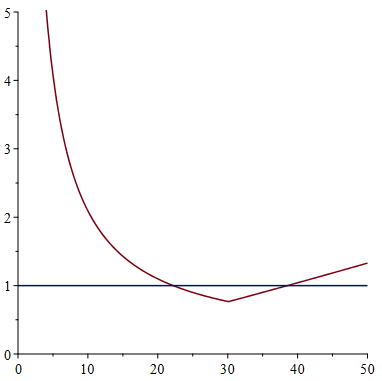
\includegraphics{dirfunc.png}
    \caption{The example direction vector over arrow-fly-time}
    \label{fig:plot_dir}
\end{figure}

\subsection{Finding t}

This last problem is not trivial, however. It is a non-linear multi-dimensional function that intersects a hyperplane on value 1 multiple times (but we cannot trivially say how often, since we do not know the funtion's behaviour). Of course we could do a lot of analysis to find out what the function looks like with different values. The problem is the high dimension of the function: We can change our position (three parameters), the position of the enemy (another three parameters), the speed of the arrow (although we could ignore that if we would say that we don't want to shoot arrows when the bow is not fully charged), the enemy's motion (three parameters again) and so on. Since we can not visualize functions with more than 2 dimensions (plus the result value mapped onto the third dimension) reasonably (but we would have at least 10 dimensions here), it would be a waste of time. This is, because we do not really need the knowledge of the function to solve the last problem:

Due to the non-linear nature of the function, we want to use a numerical approach anyway. And those approaches tend to be useful on a variety of problems. For our scenario two algorithms seem to be fitting: Newton's method for solving non-linear equation systems or the Bisection algorithm that is a common way to find the root of a number.

Actually, there is a third way which is by far less elegant but much easier to implement: We could just test the function with integer values - let's say from 0 to 200 (the latter would be a ten-second-flight-time, so we do not really need to test further). This would be a waste of calculation time, but less error prone and not especially painful, since the function is not too hard to compute.

The Newton algorithm works like this: We start at a safe value (something around 1 or 2 because before that we have the problem, that the function has tremendously high values - that would be inconvenient) and calculate the derivate with respect to time. Of course we fix the values for position, angle vector, velocity and so on, since in the scenario of the calculation they are already known (unlike during analysis) so the function has only two dimensions left: Flight time and length of the angle vector. The derivate is easy to calculate because we do only need the derivate at the chosen point, so we can just use the approximate gradient of the function at the given point. Then, we use the result of that to construct a tangent and search for the intersection of the tangent with our hyperplane (which is a line at value 1). Then we take the x-value of that intersection and repeat the process all over again, until we reach a point close enough to 1.

The Bisect algorithm is a little bit easier: We take any x-value (where we know the function is above 1) and any other value (where we know the function is beneath 1) and take the middle of those values. Then we calculate the functions result at this middle point and adjust our interval in a way, that the intersection with our hyperplane is still within the interval. We do repeat this process until we find a point close enough to 1. 

Since the Newton algorithm can potentially fail (because as we can see in \figurename{} \ref{fig:plot_dir} the function is not smooth) but we do not know values to start with for the Bisect algorithm, I would combine those two. Use Newton to find starting values for Bisect and then use Bisect to find the intersection. Then we take the y-value of the function and now we can calculate the direction where to shoot at, since we have a valid value for $t$ in our formula.